
Теперь посмотрим на поведение характеристик в зависимости от параметров построения графов, при фиксированных распределениях
\\
\begin{equation*}
    \text{Laplace}(\ 0, \frac{1}{\sqrt{2}}) \qquad\qquad Skewnormal (1)
\end{equation*}
\textbf{Графики для KNN графа :}


\hspace*{-1cm}
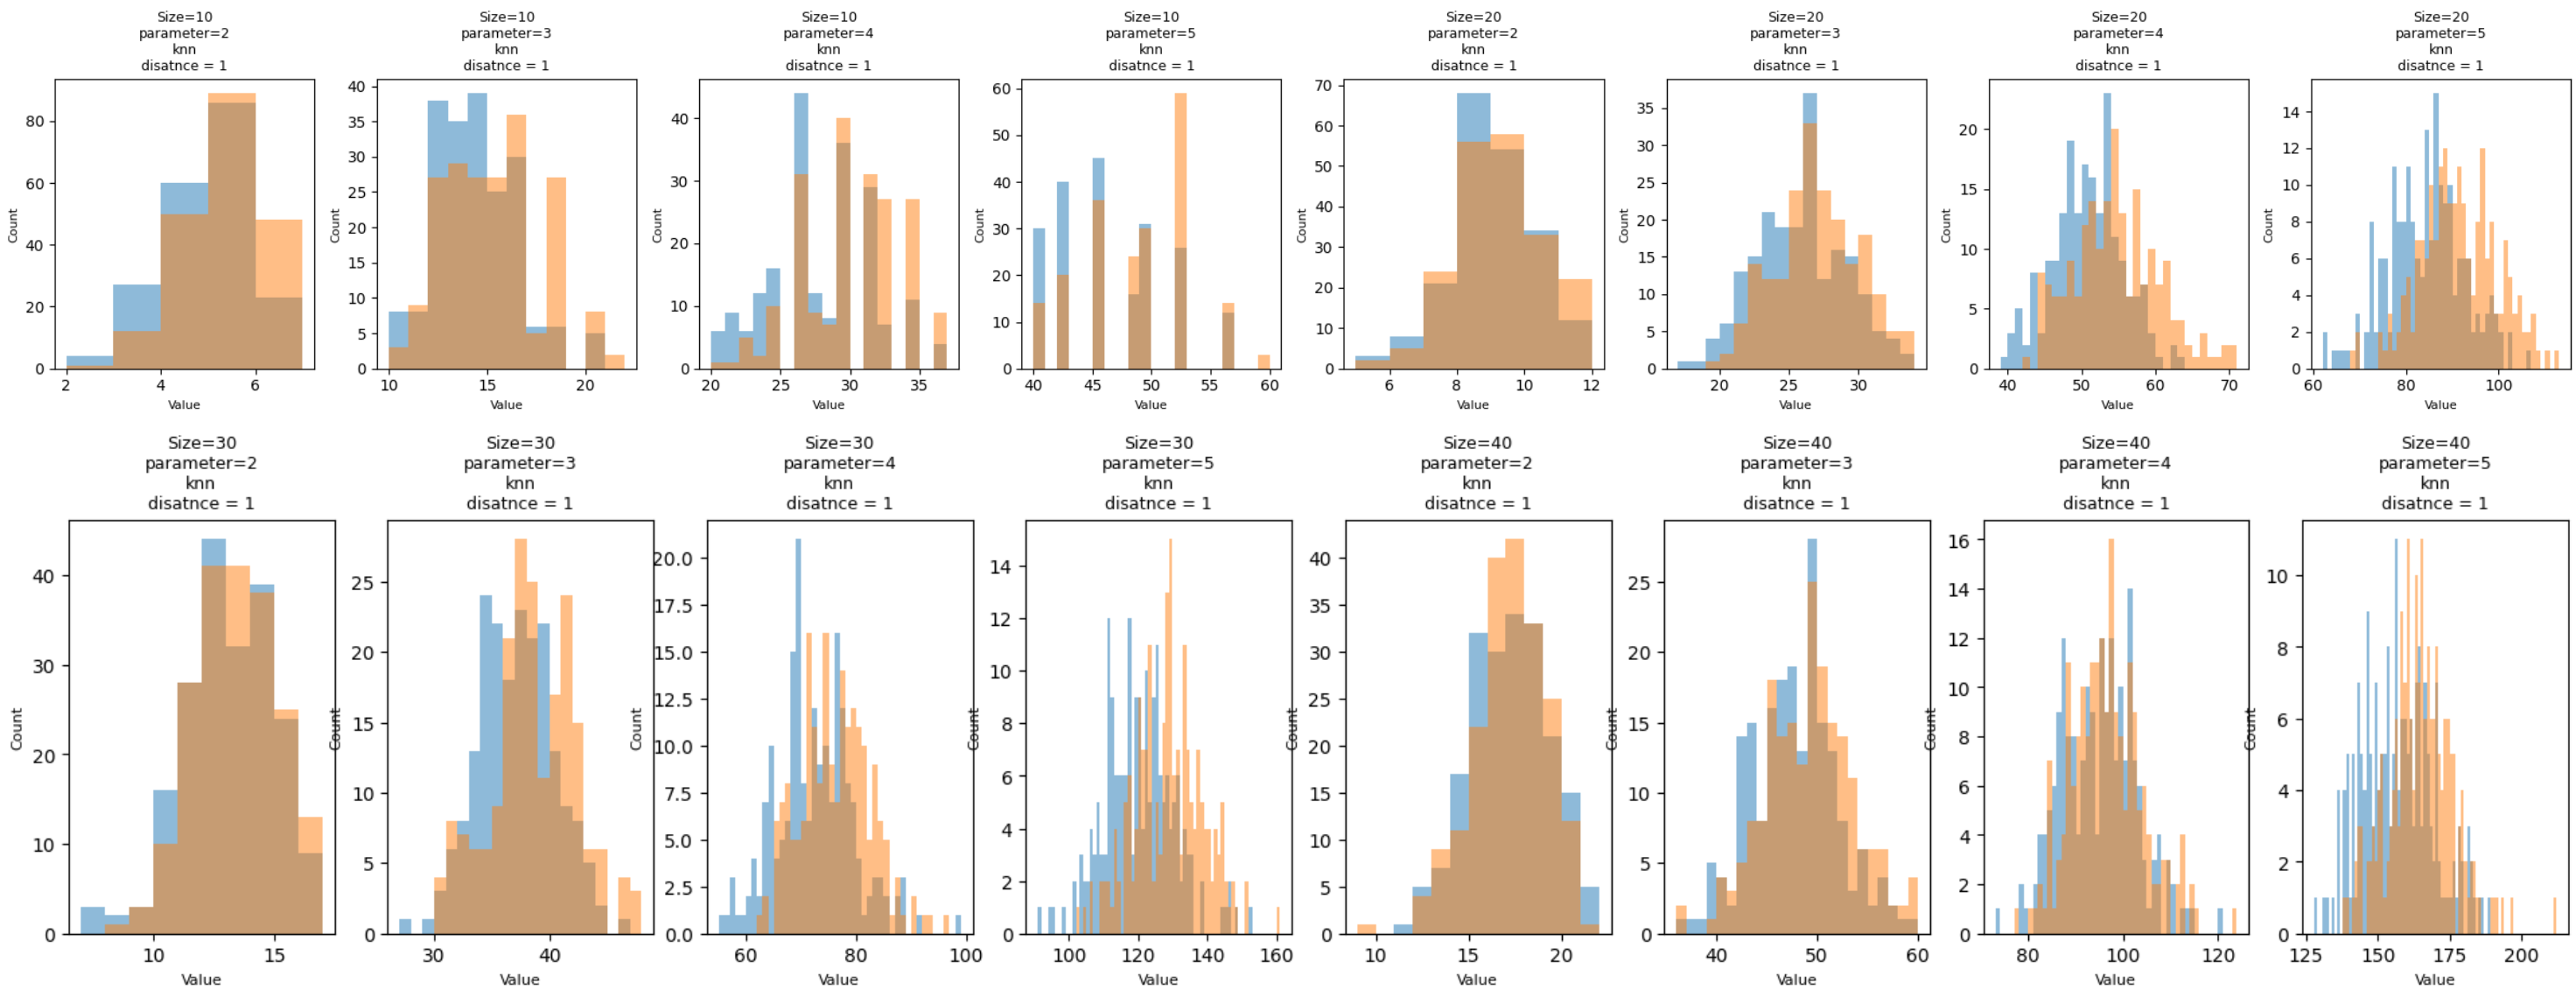
\includegraphics[width=1\textwidth]{Part-I-Ivanova/2_1_hist.png}

\noindent\textbf{Вывод:} При любом размере выборки количество треугольников не выглядит хорошей характеристикой, потому что графики практически идентичны. Лучшее, что можно получить, при количестве вершин 40 и количестве соседей в графе - 5 (правый нижний график)
\\
\noindent\textbf{Графики для дистанционного графа}
\\
\hspace*{-0.5cm}
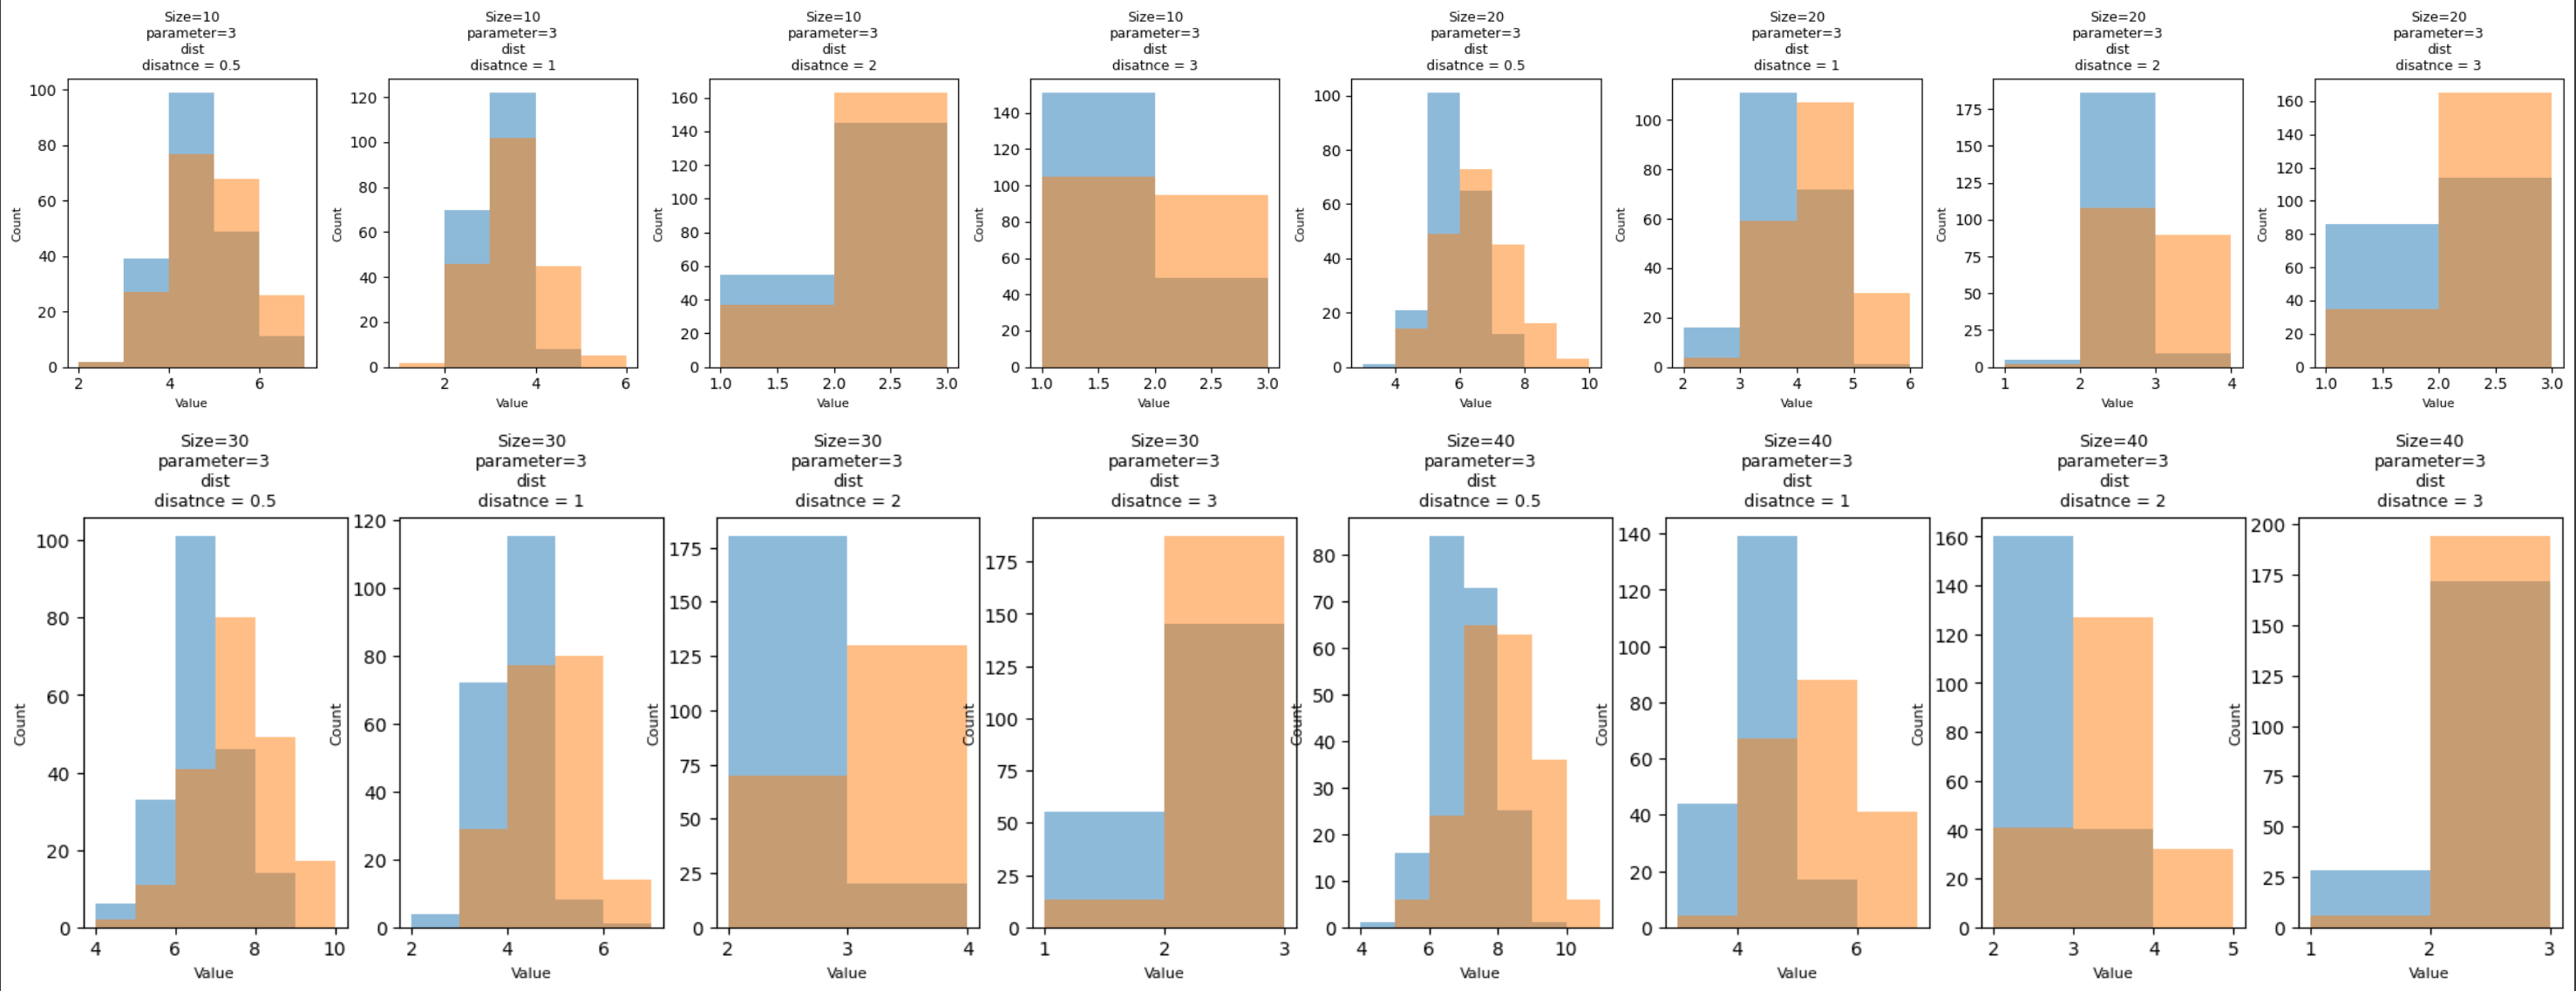
\includegraphics[width=1\textwidth]{Part-I-Ivanova/2_2_hist.png}\\ 


\noindent \textbf{Вывод:} Максимальное независимое множество, с точки зрения задачи классификации, для данных распределений является признаком получше, например для 40 вершин и дистанции 2, распределения уже неплохо различимы, на основе этой характеристики и будем строить критическое множество. 
